\clearpage
\section{Data control region plots}
\label{sec:data-control-region-plots}

Monte Carlo simulation is being used in this analysis both to train the \glspl{bdt} and to gain understanding of the composition of the standard model processes in the background. It is therefore useful to compare data and simulation plots to verify that the simulation does not significantly diverge from the data. However, to avoid unblinding the data in sensitive regions, the comparison plots are done in a \gls{cr}. A straightforward \gls{cr} is the same as the normalization region for the background estimation methods of $\text{BDT} < 0$. For this study, the most sensitive category, namely the dimuon category, was chosen. The data taking period used is tracker phase 1, which has higher luminosity and is expected to suffer from some data quality issues that are further addressed in Section~\ref{sec:data-quality}. The simulation has been normalized for phase 1 luminosity, and the comparison plots can be seen in Figure~\ref{fig:data-control-plots-dimuon-phase1}. Good agreement between data and simulation can be observed in the ratio panel.


\begin{figure}[!htb]
\centering
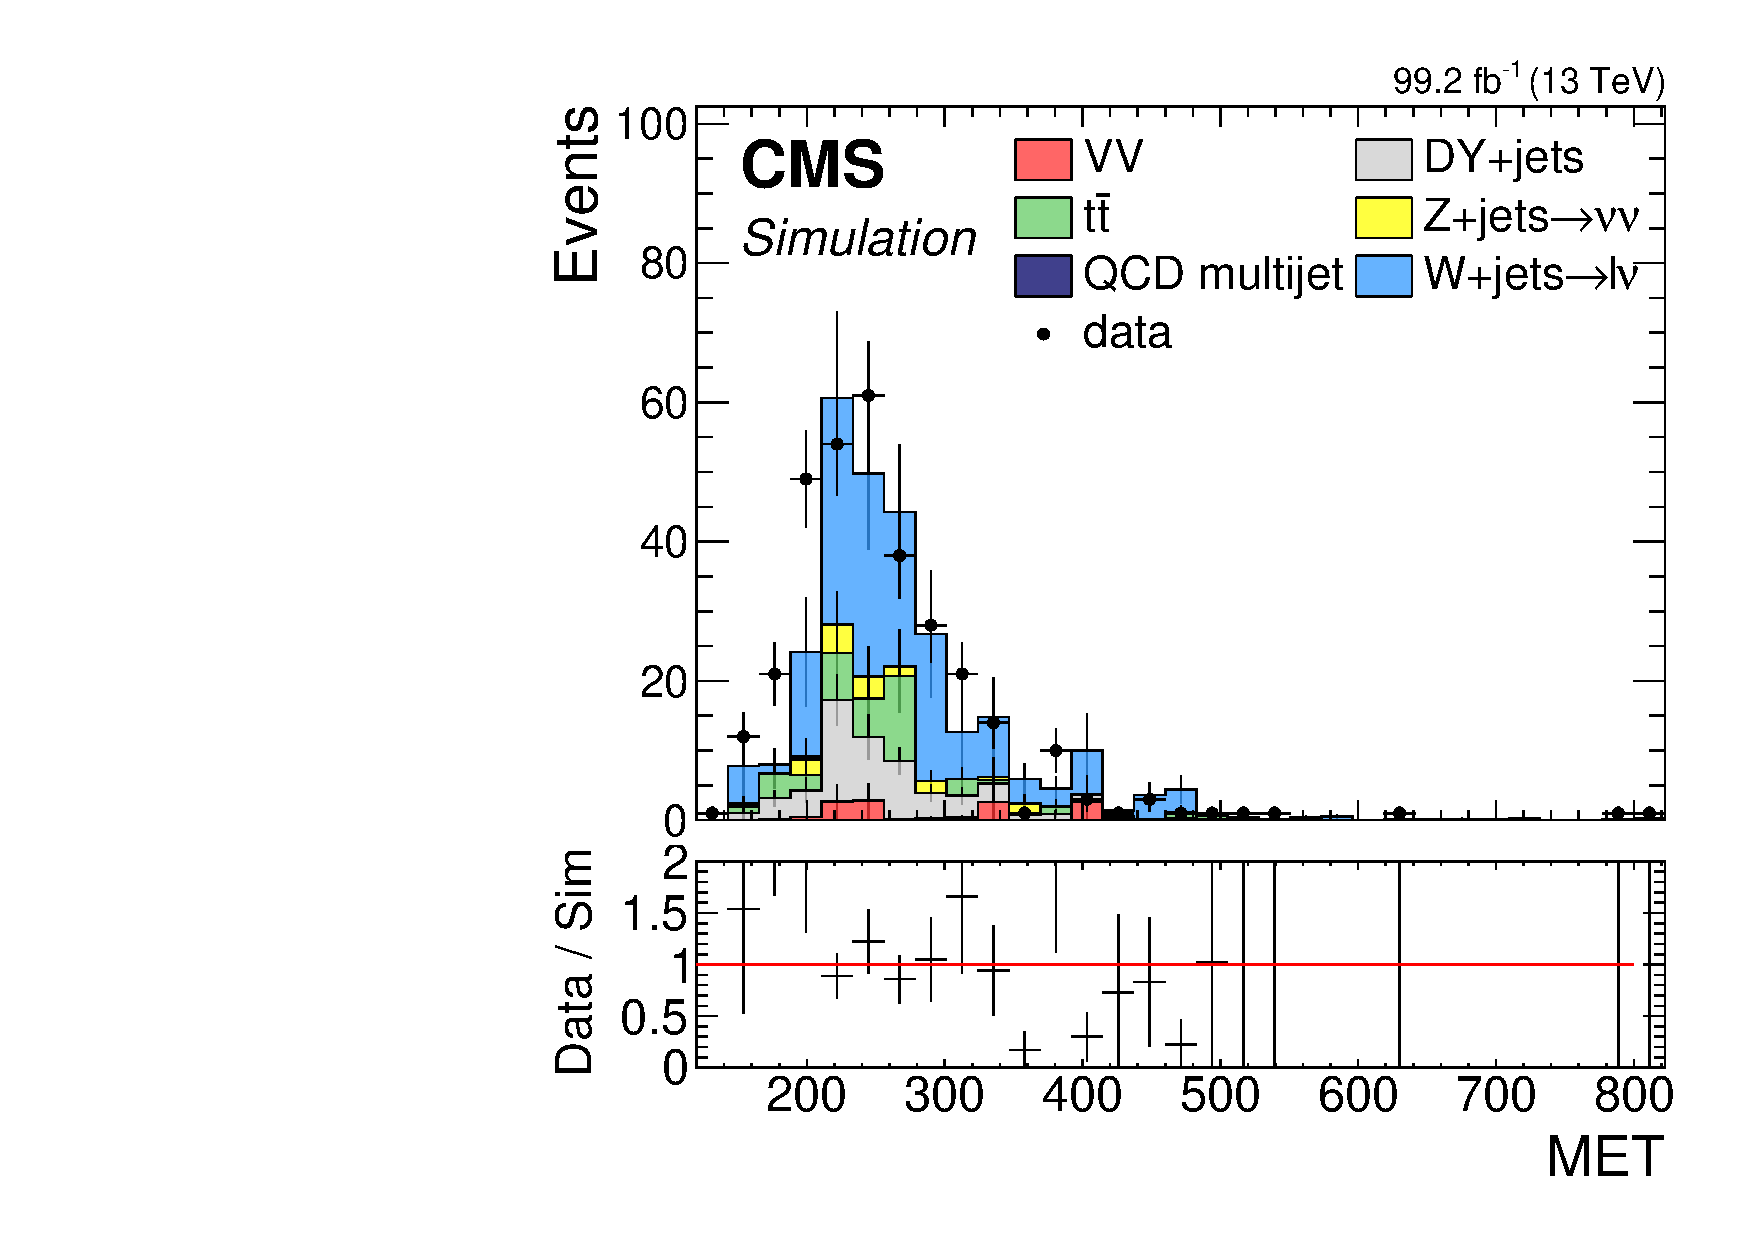
\includegraphics[width=0.48\linewidth]{plots/dilepton_muons_data_control_region_phase1/none_MET.pdf} \,
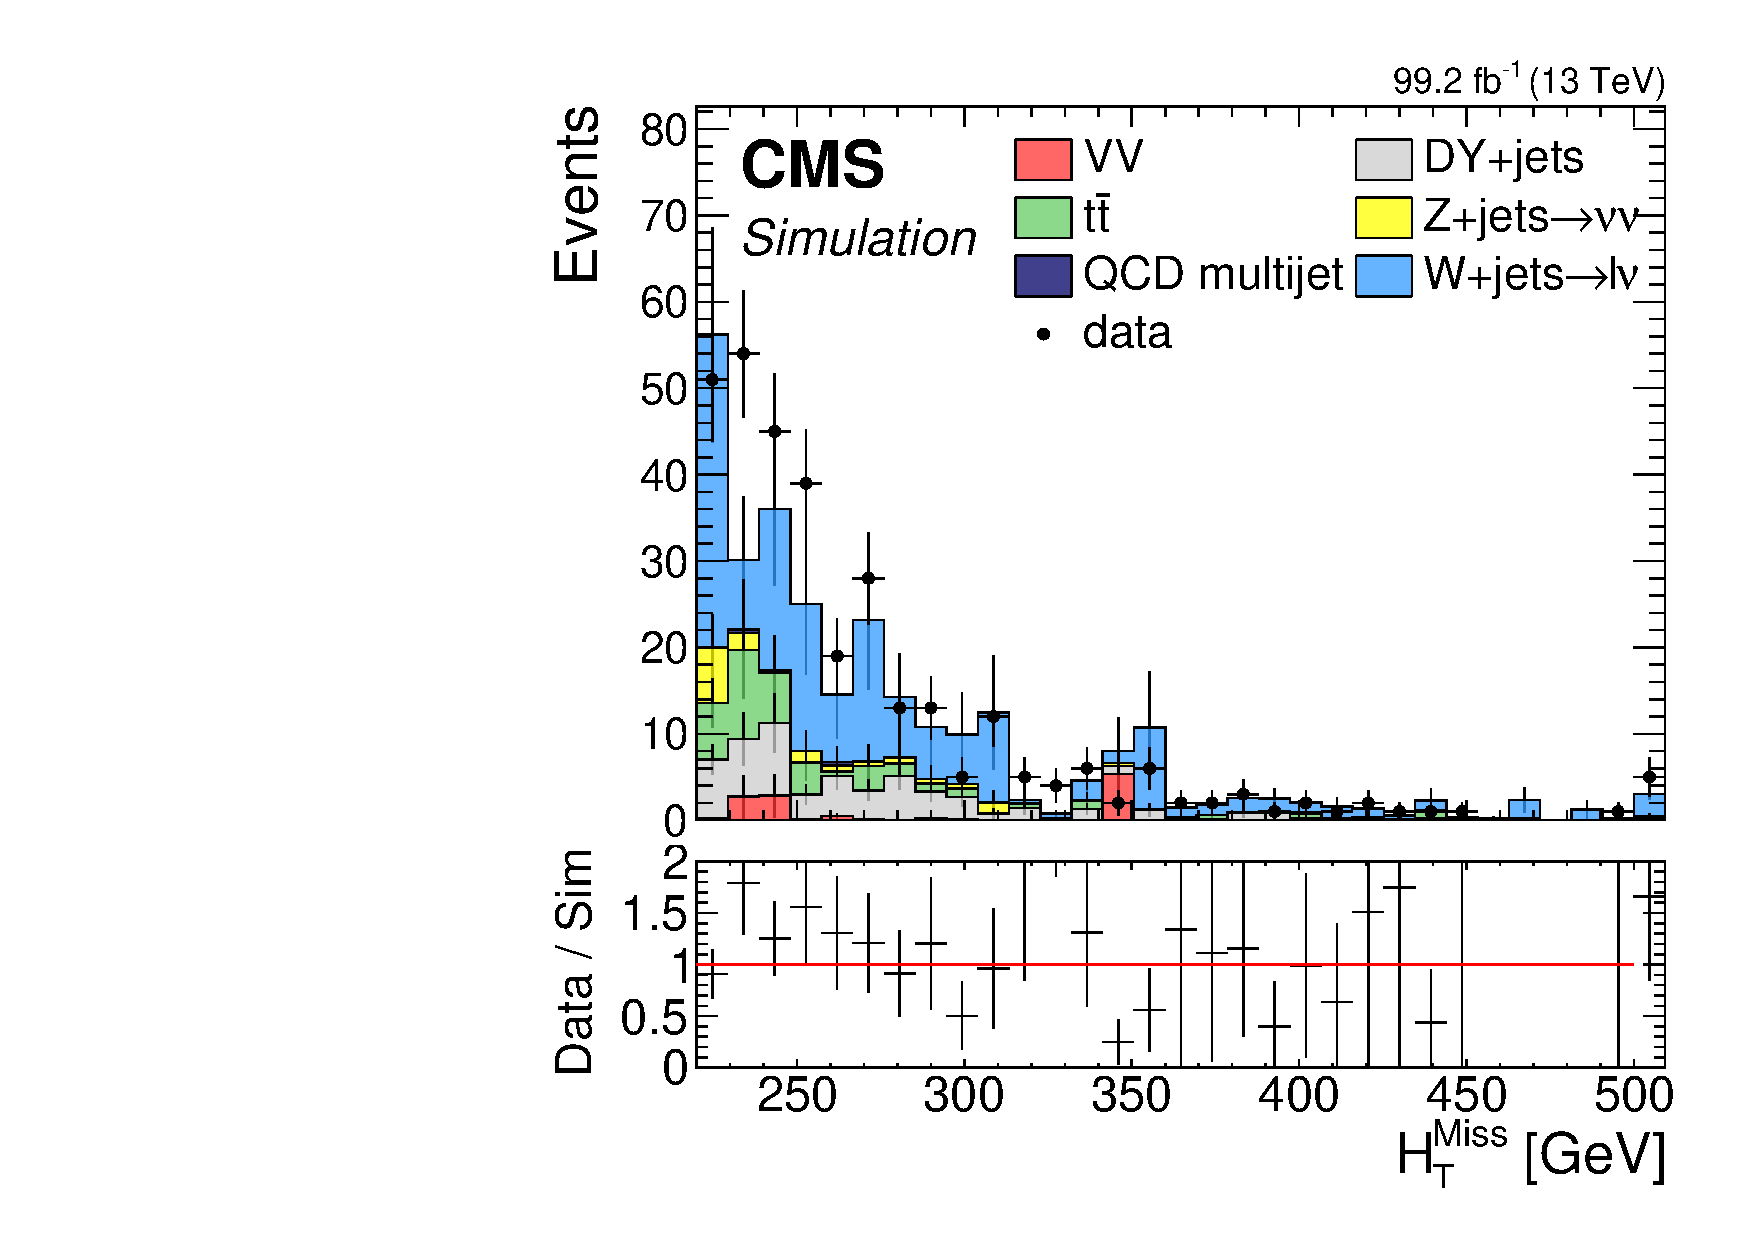
\includegraphics[width=0.48\linewidth]{plots/dilepton_muons_data_control_region_phase1/none_MHT.pdf} \\

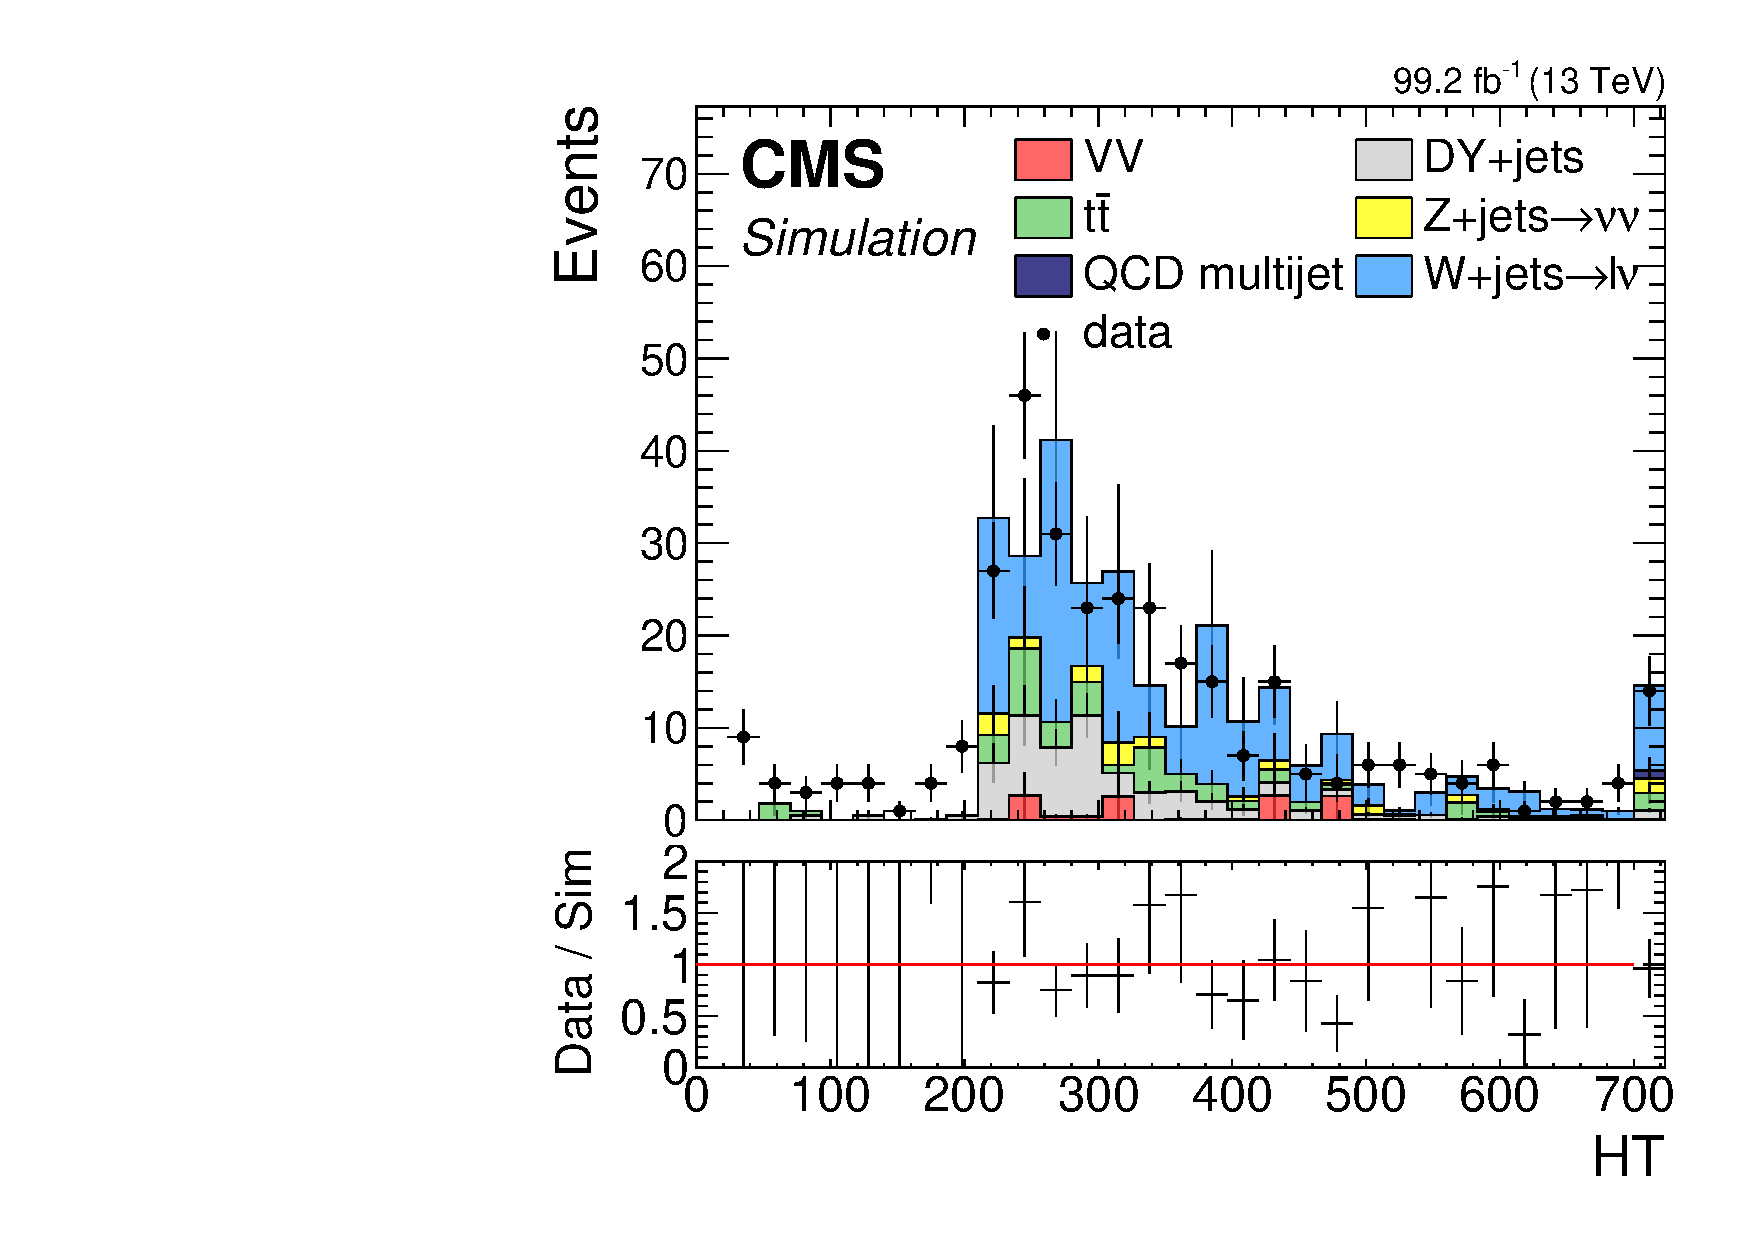
\includegraphics[width=0.48\linewidth]{plots/dilepton_muons_data_control_region_phase1/none_HT.pdf} \,
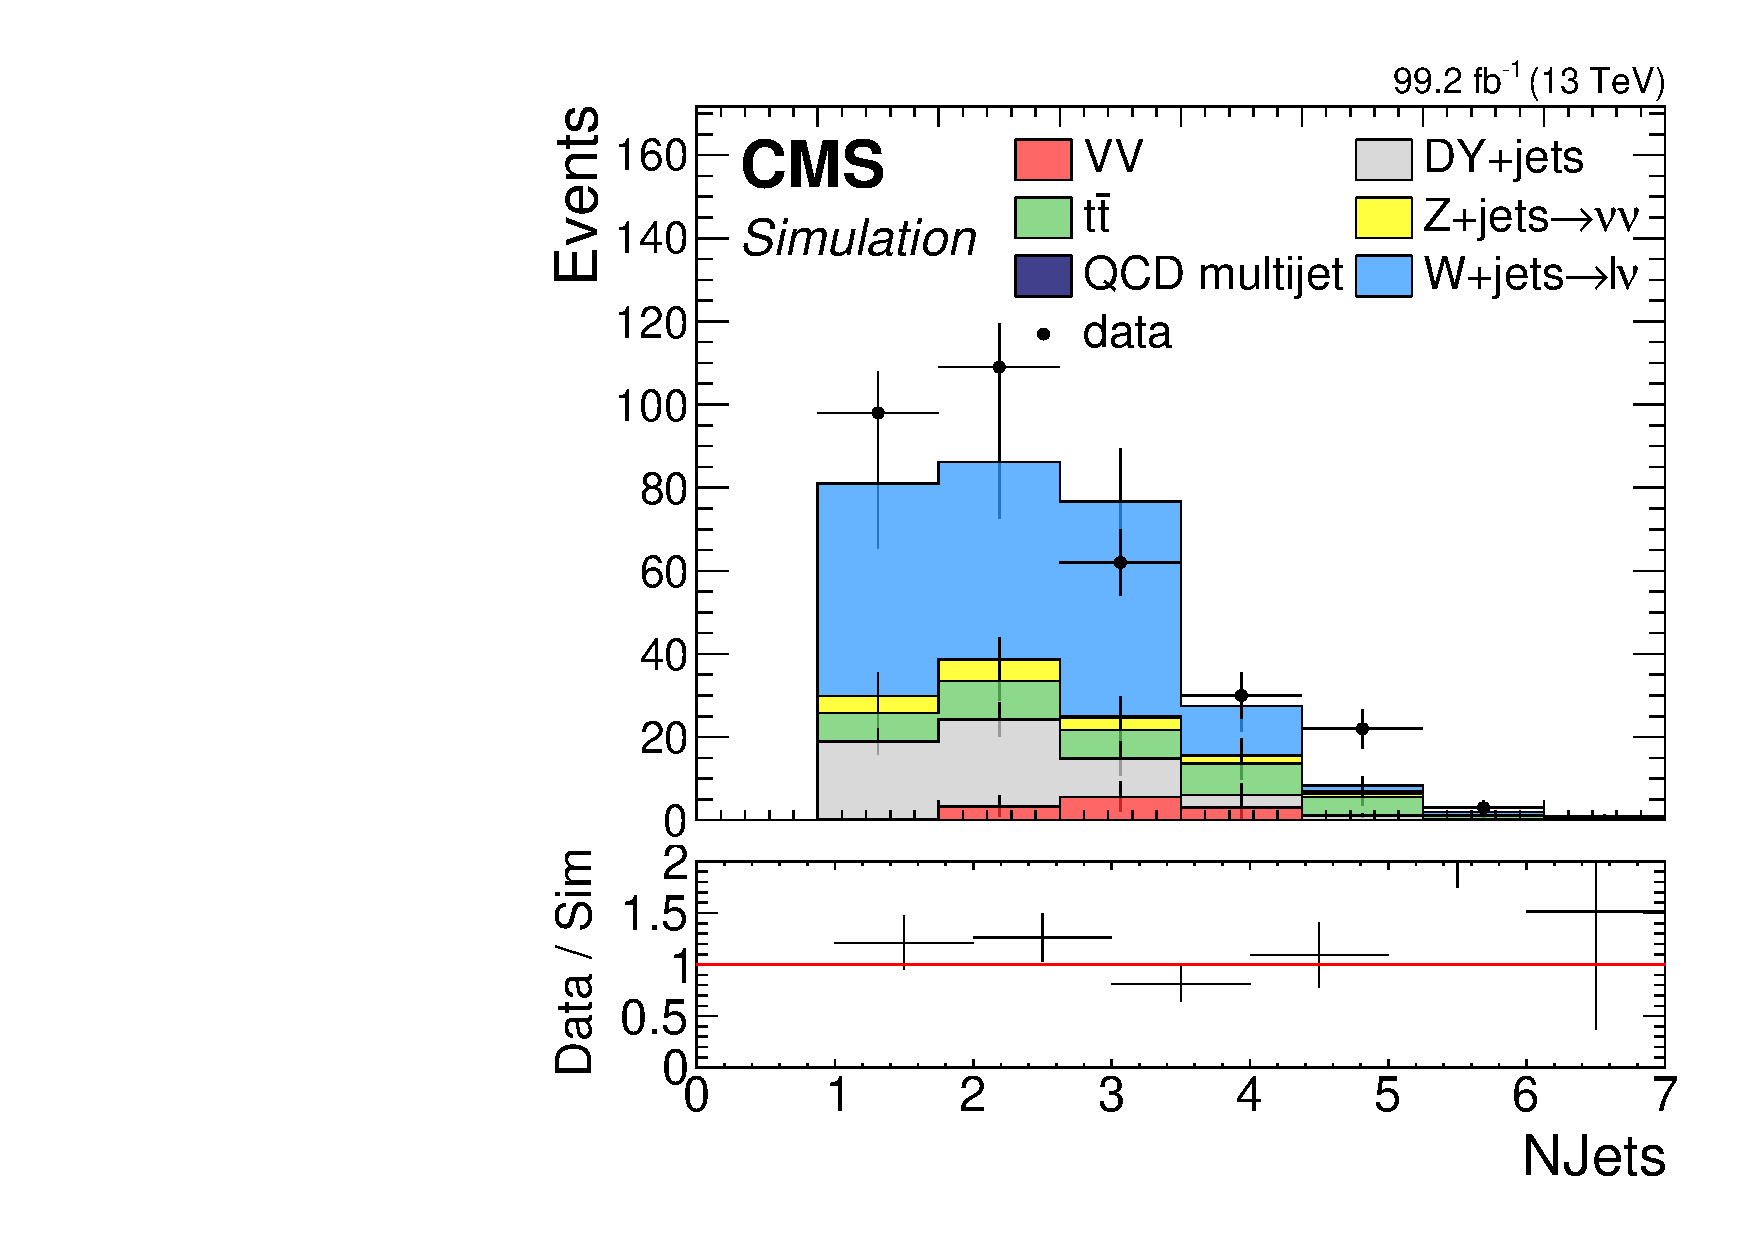
\includegraphics[width=0.48\linewidth]{plots/dilepton_muons_data_control_region_phase1/none_NJets.pdf} \\

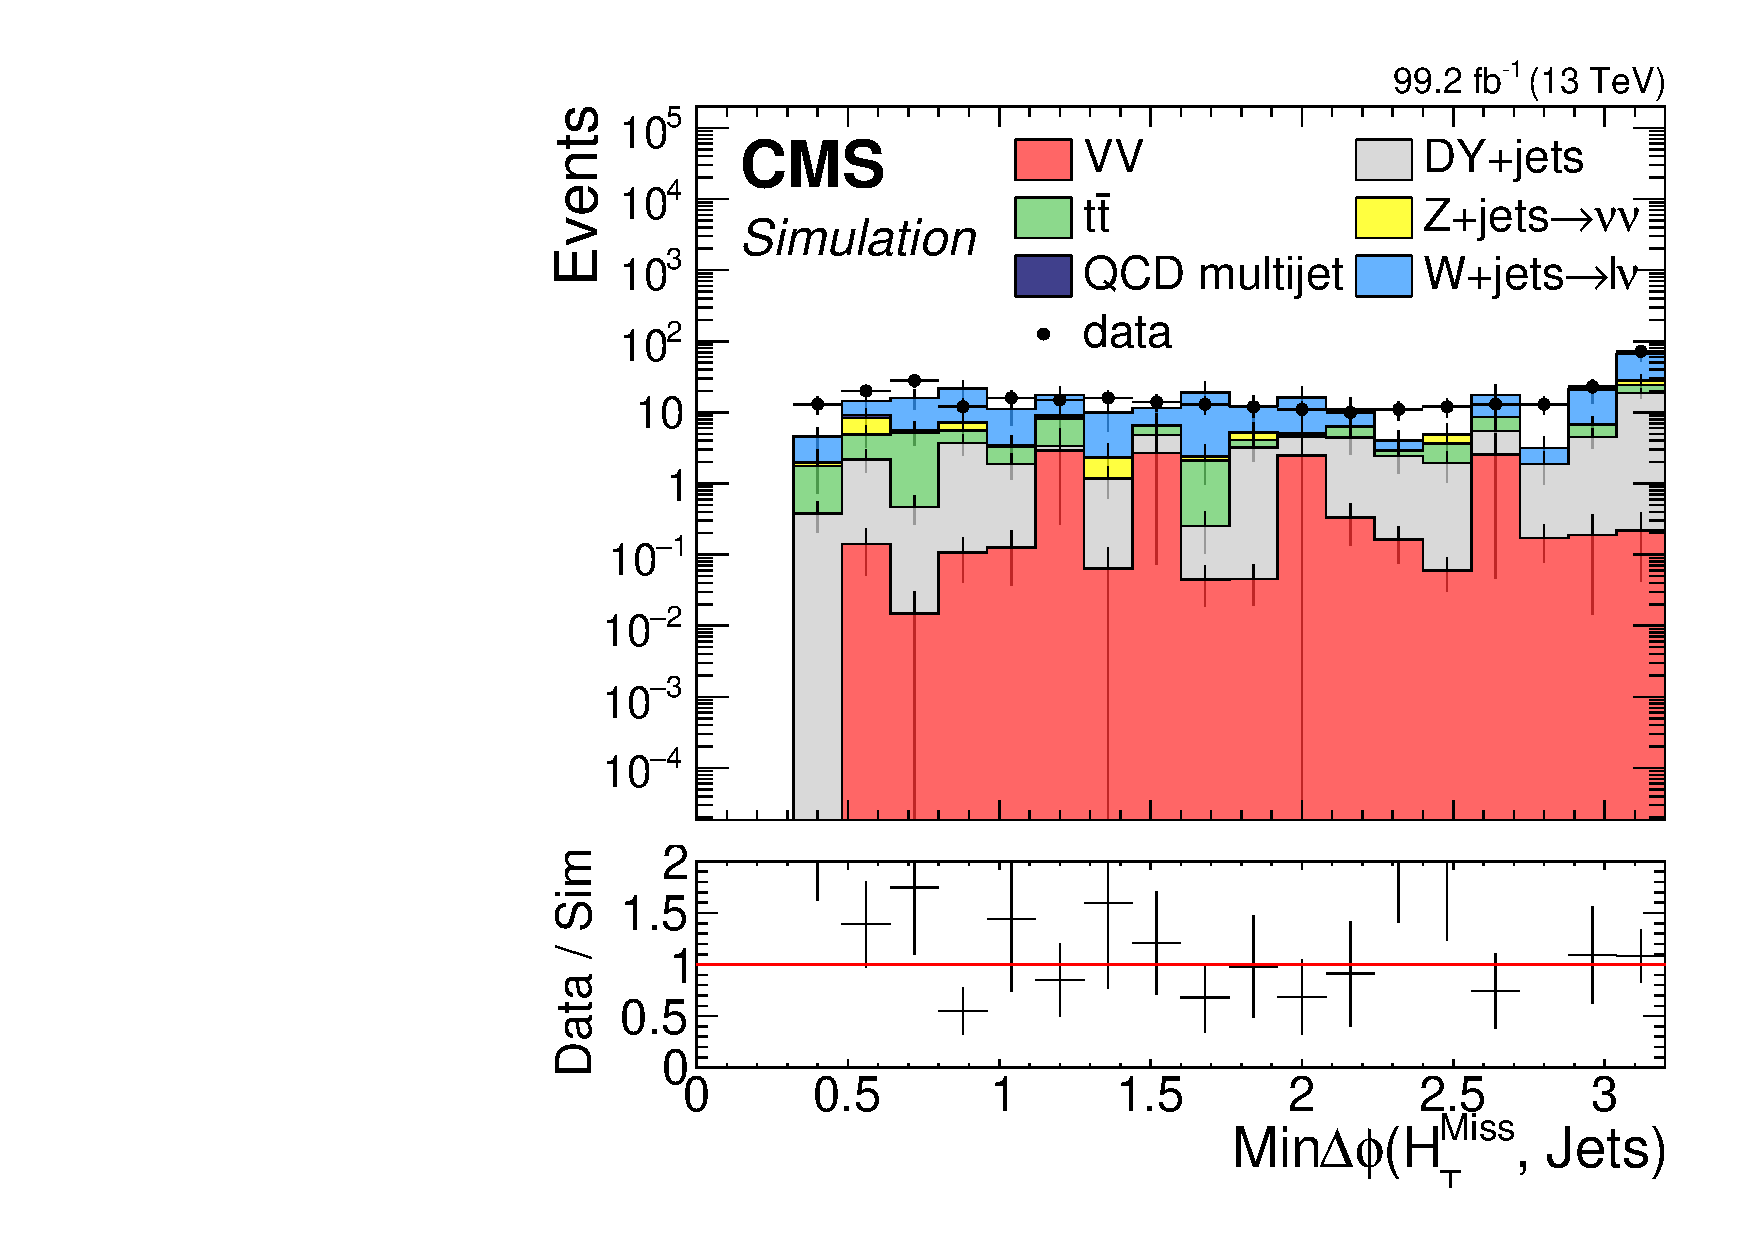
\includegraphics[width=0.48\linewidth]{plots/dilepton_muons_data_control_region_phase1/none_MinDeltaPhiMhtJets_log.pdf} \,
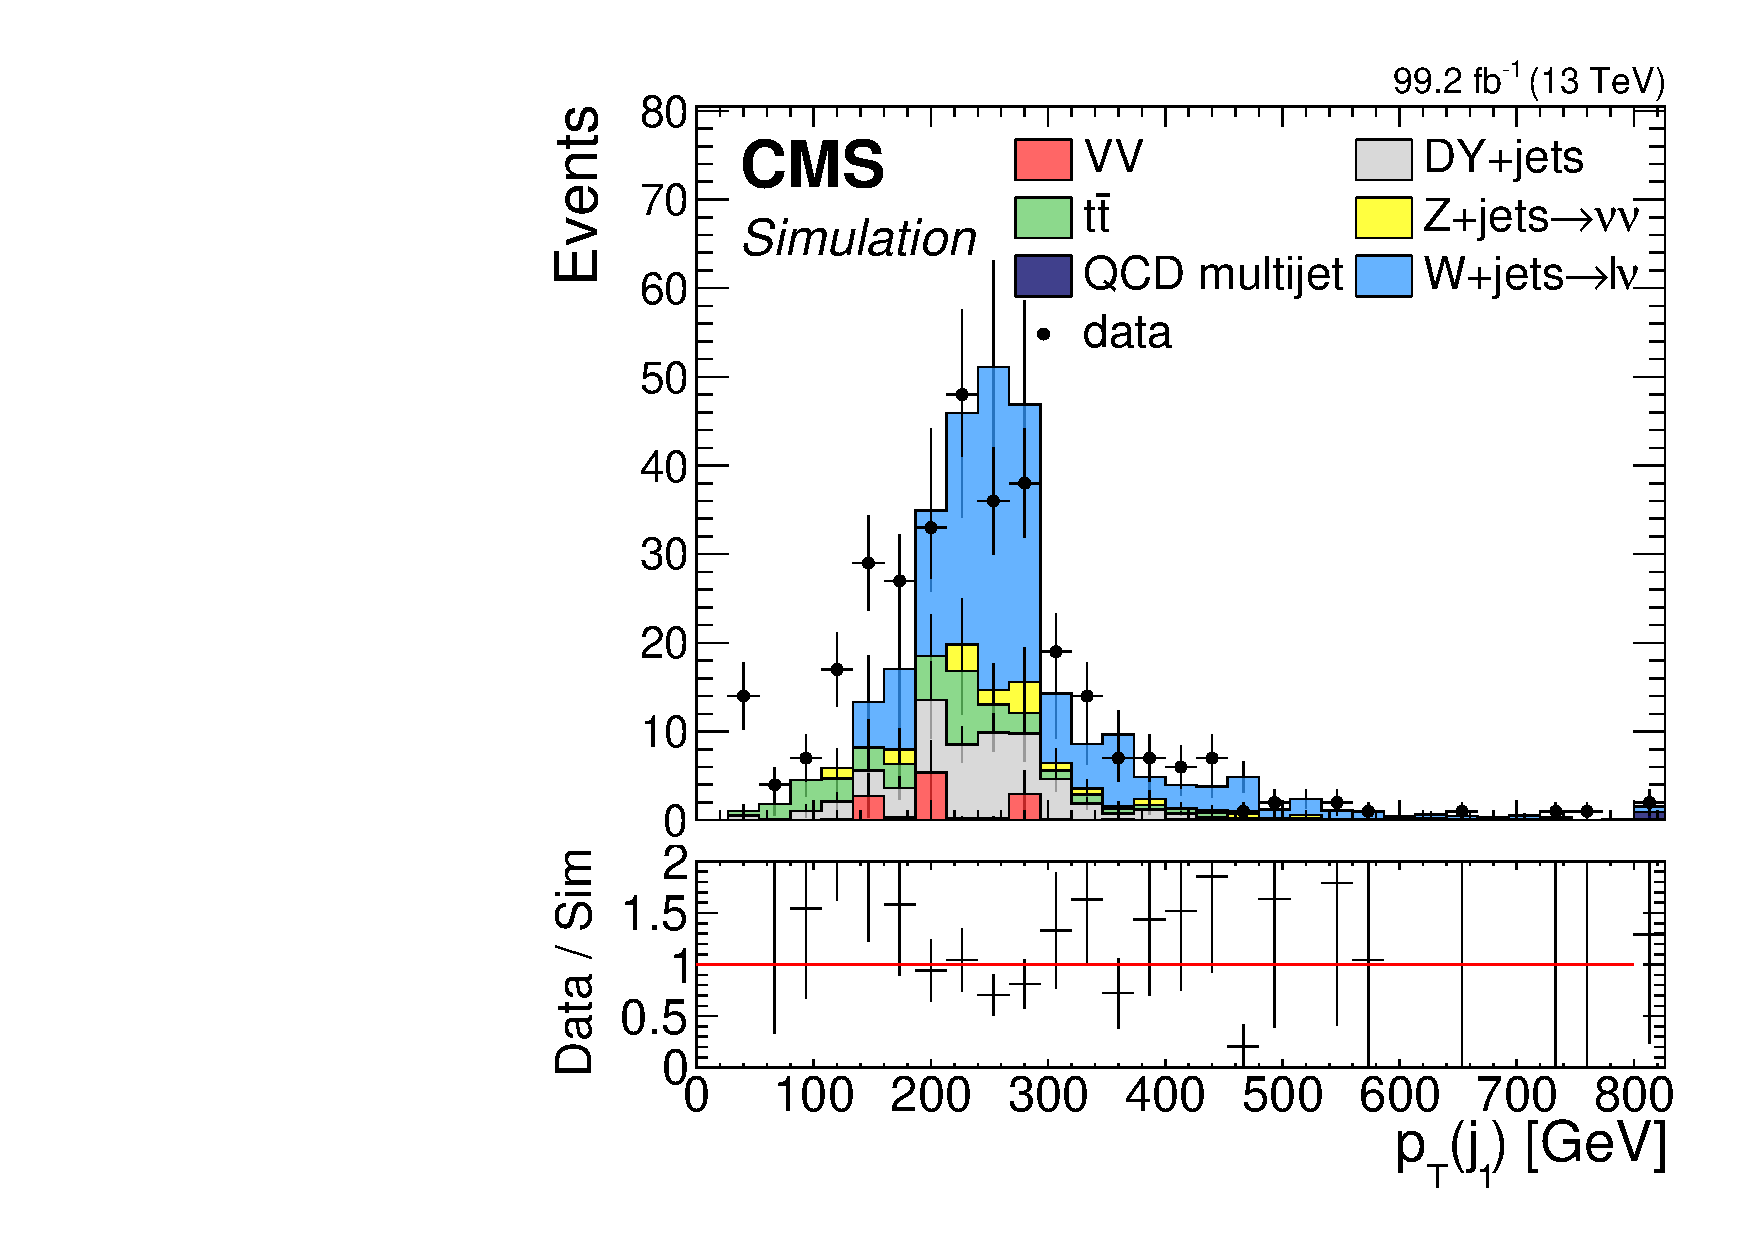
\includegraphics[width=0.48\linewidth]{plots/dilepton_muons_data_control_region_phase1/none_LeadingJetPt.pdf} \\

\caption[Data control region plots for dimuon category in phase 1]{Data control region plots for dimuon category in phase 1.}
\label{fig:data-control-plots-dimuon-phase1}
\end{figure} 


\begin{figure}[!htb]
\centering
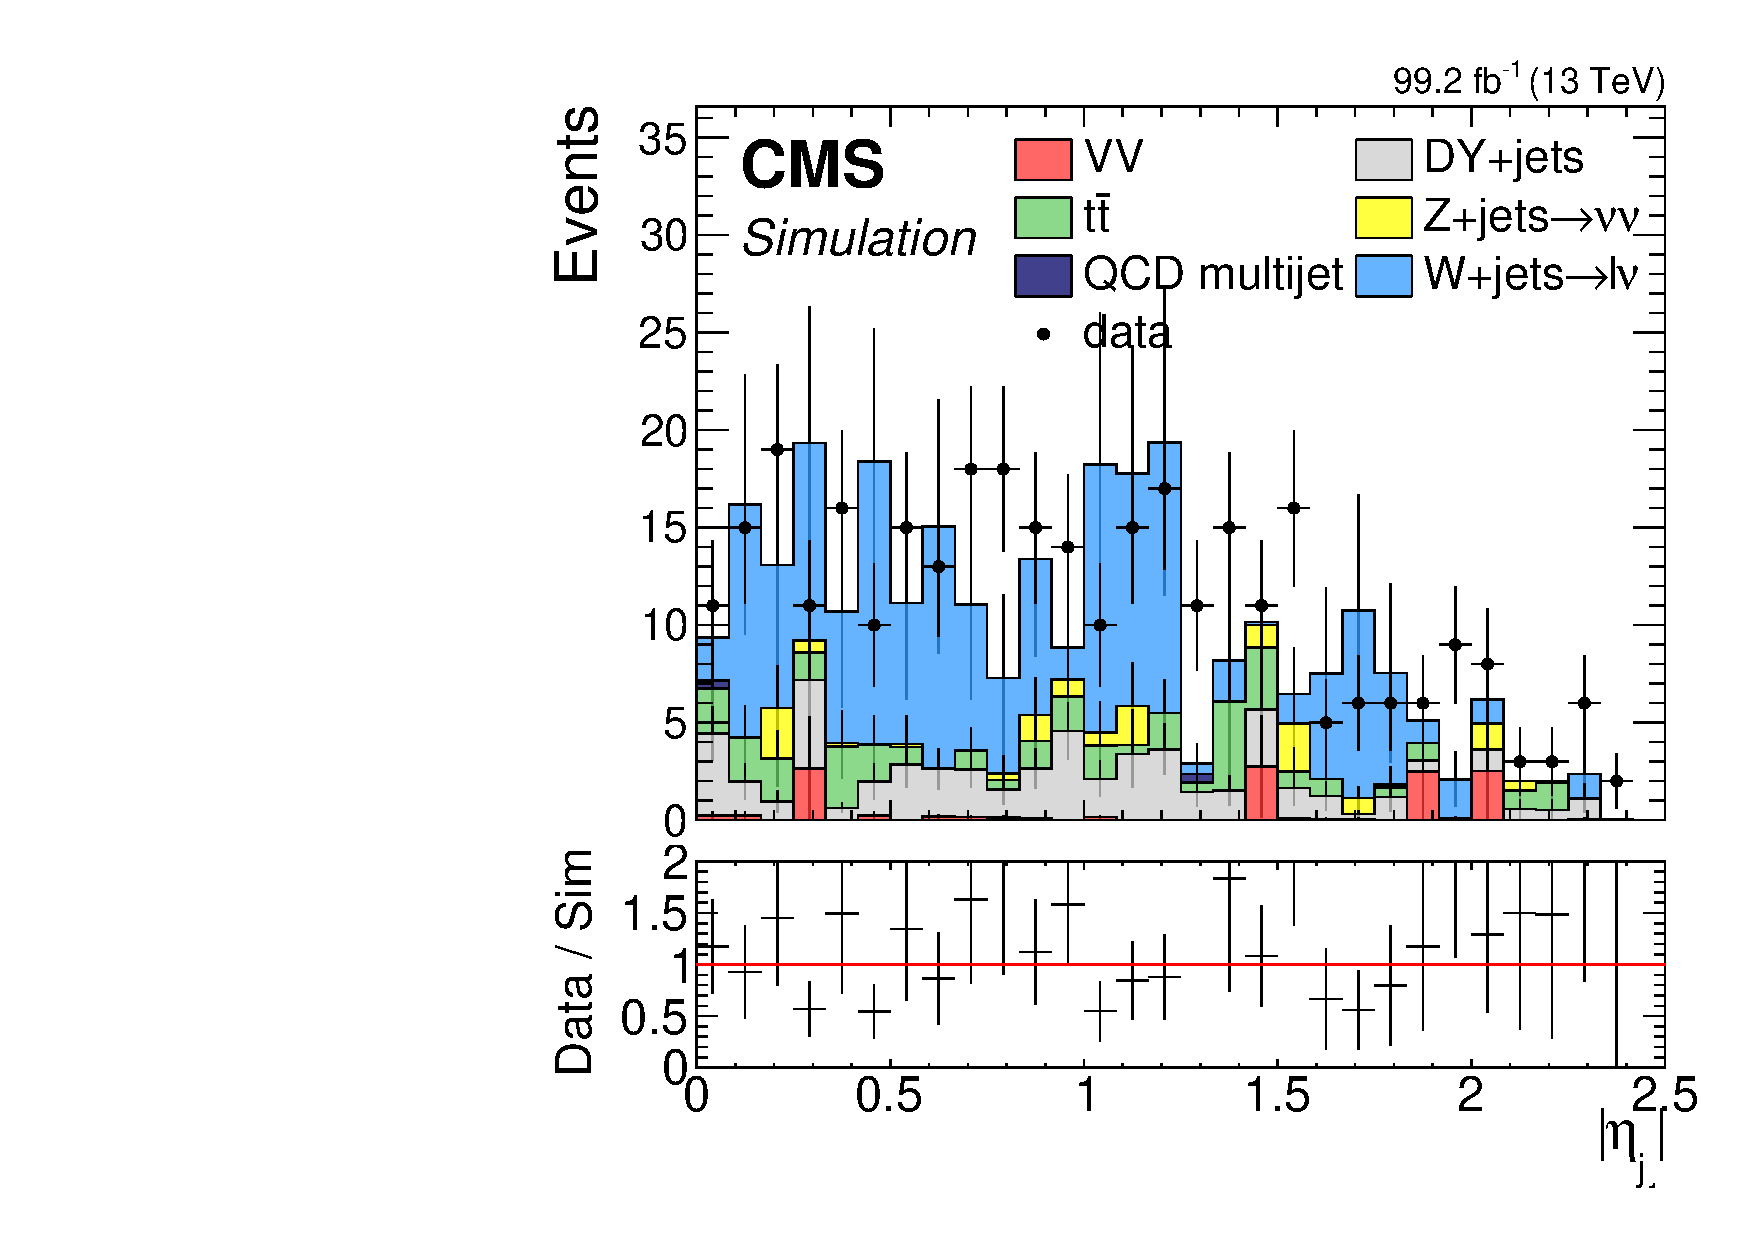
\includegraphics[width=0.48\linewidth]{plots/dilepton_muons_data_control_region_phase1/none_abs(LeadingJet.Eta()).pdf} \,
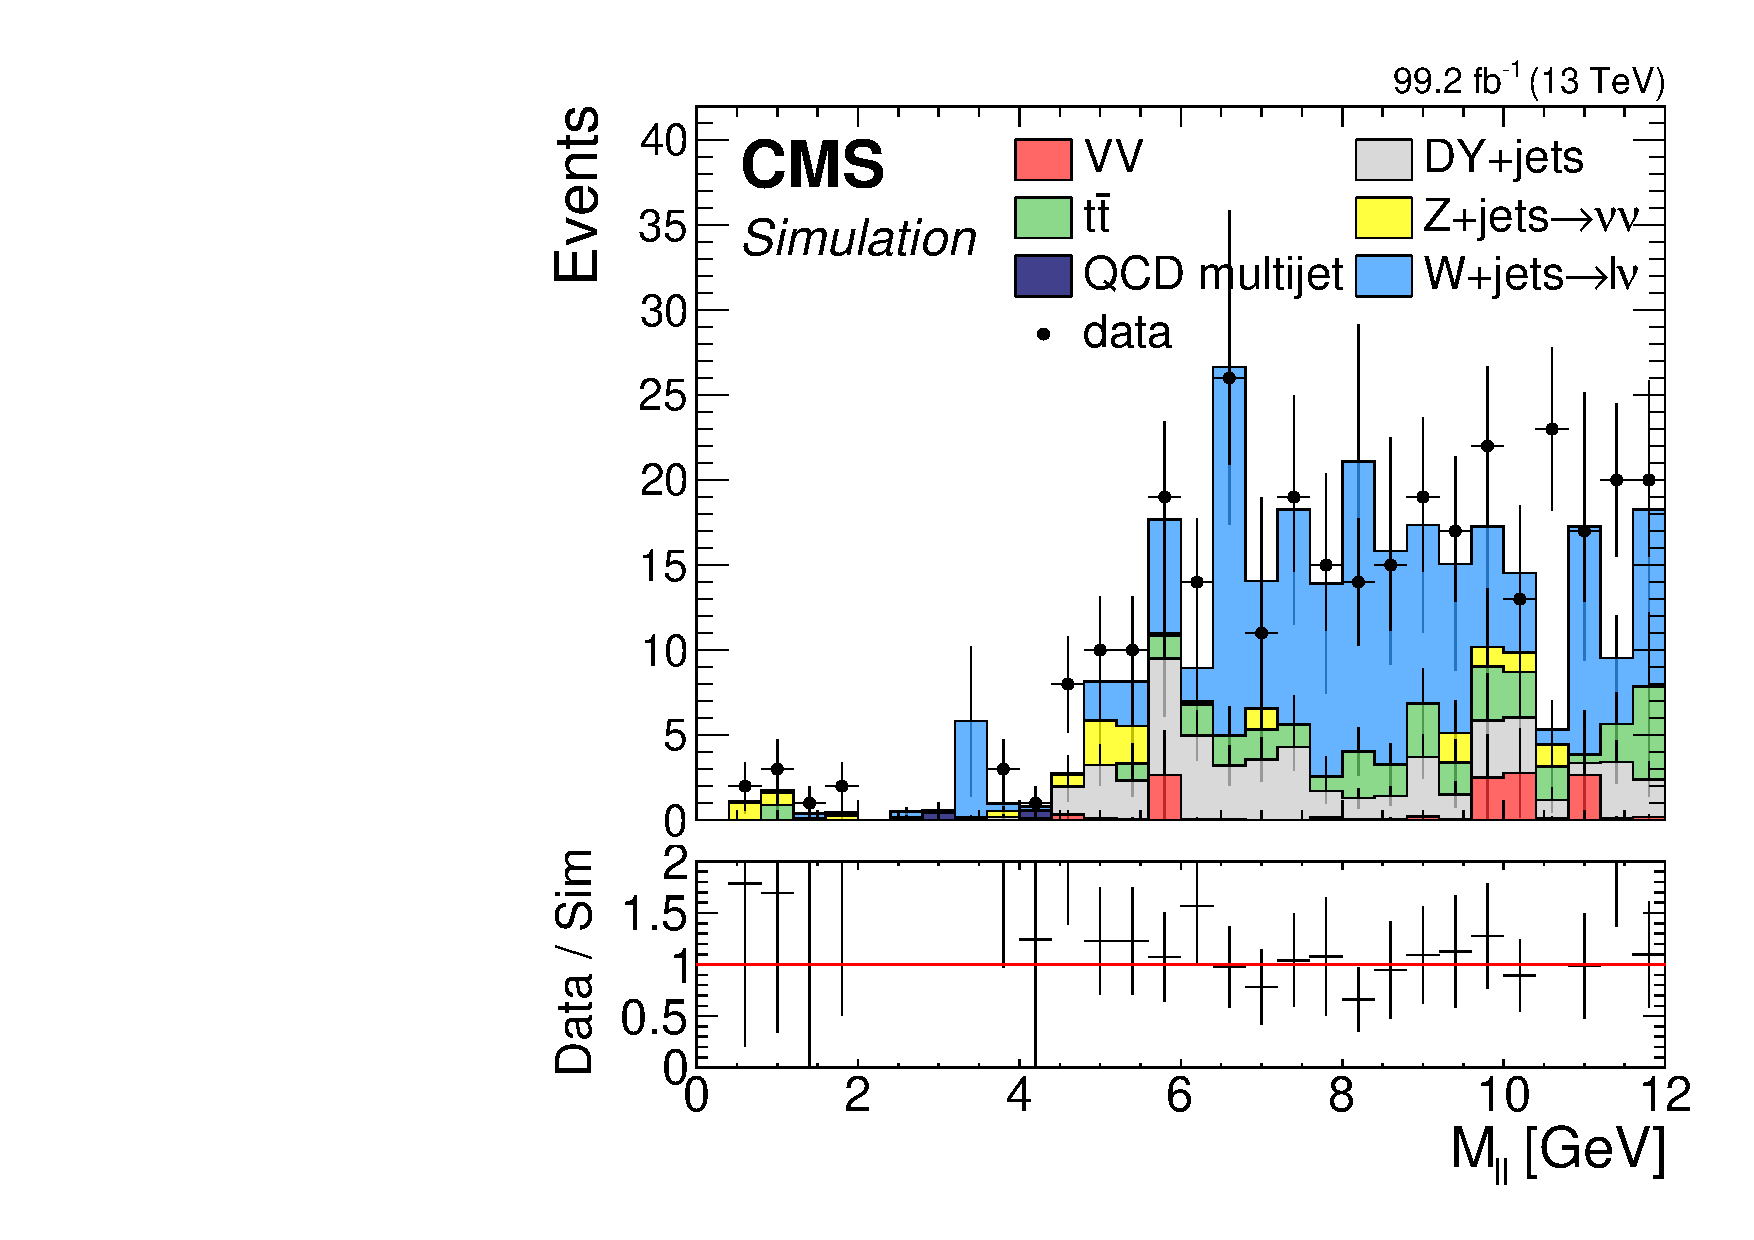
\includegraphics[width=0.48\linewidth]{plots/dilepton_muons_data_control_region_phase1/none_invMassCorrJetNoMultIso10Dr0.6.pdf} \\

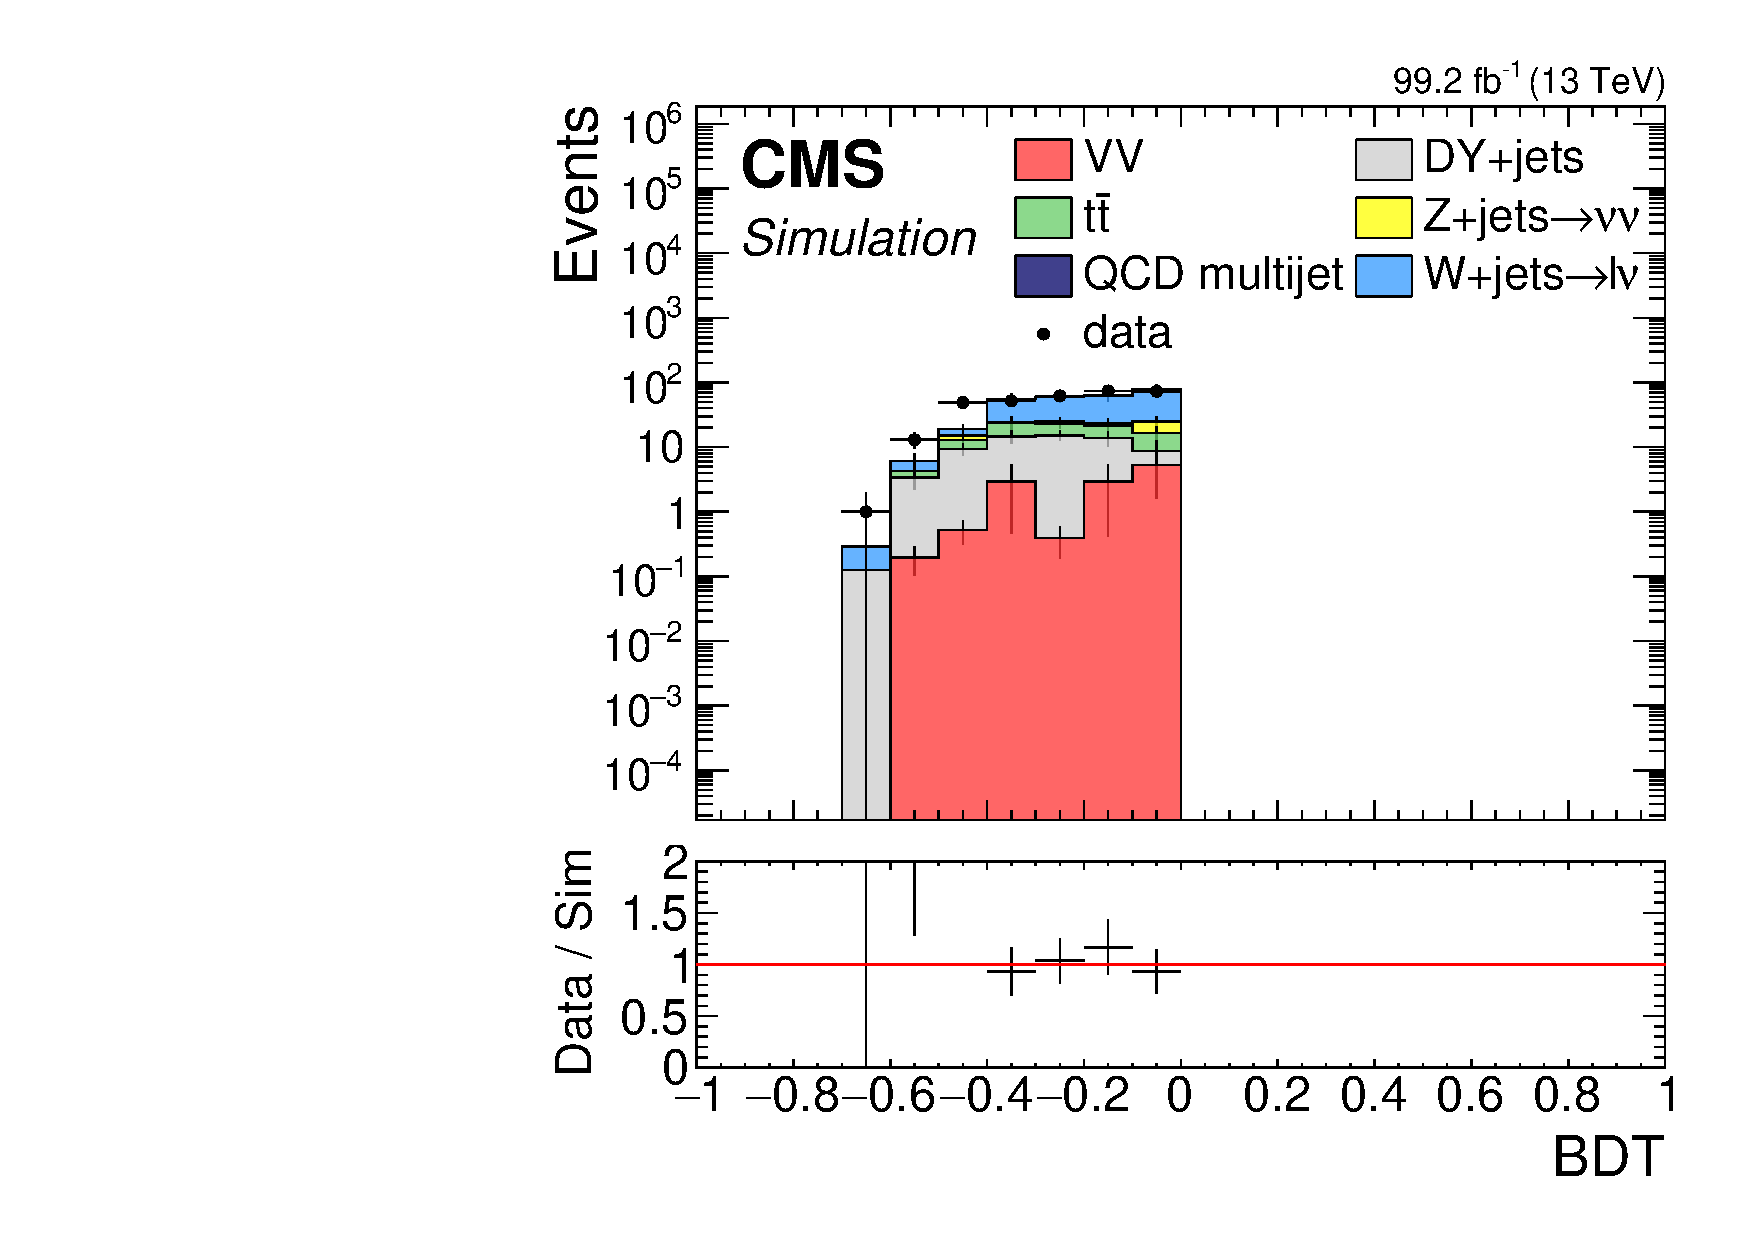
\includegraphics[width=0.48\linewidth]{plots/dilepton_muons_data_control_region_phase1/none_custom_dilepBDTCorrJetNoMultIso10Dr0.6_log.pdf} \,
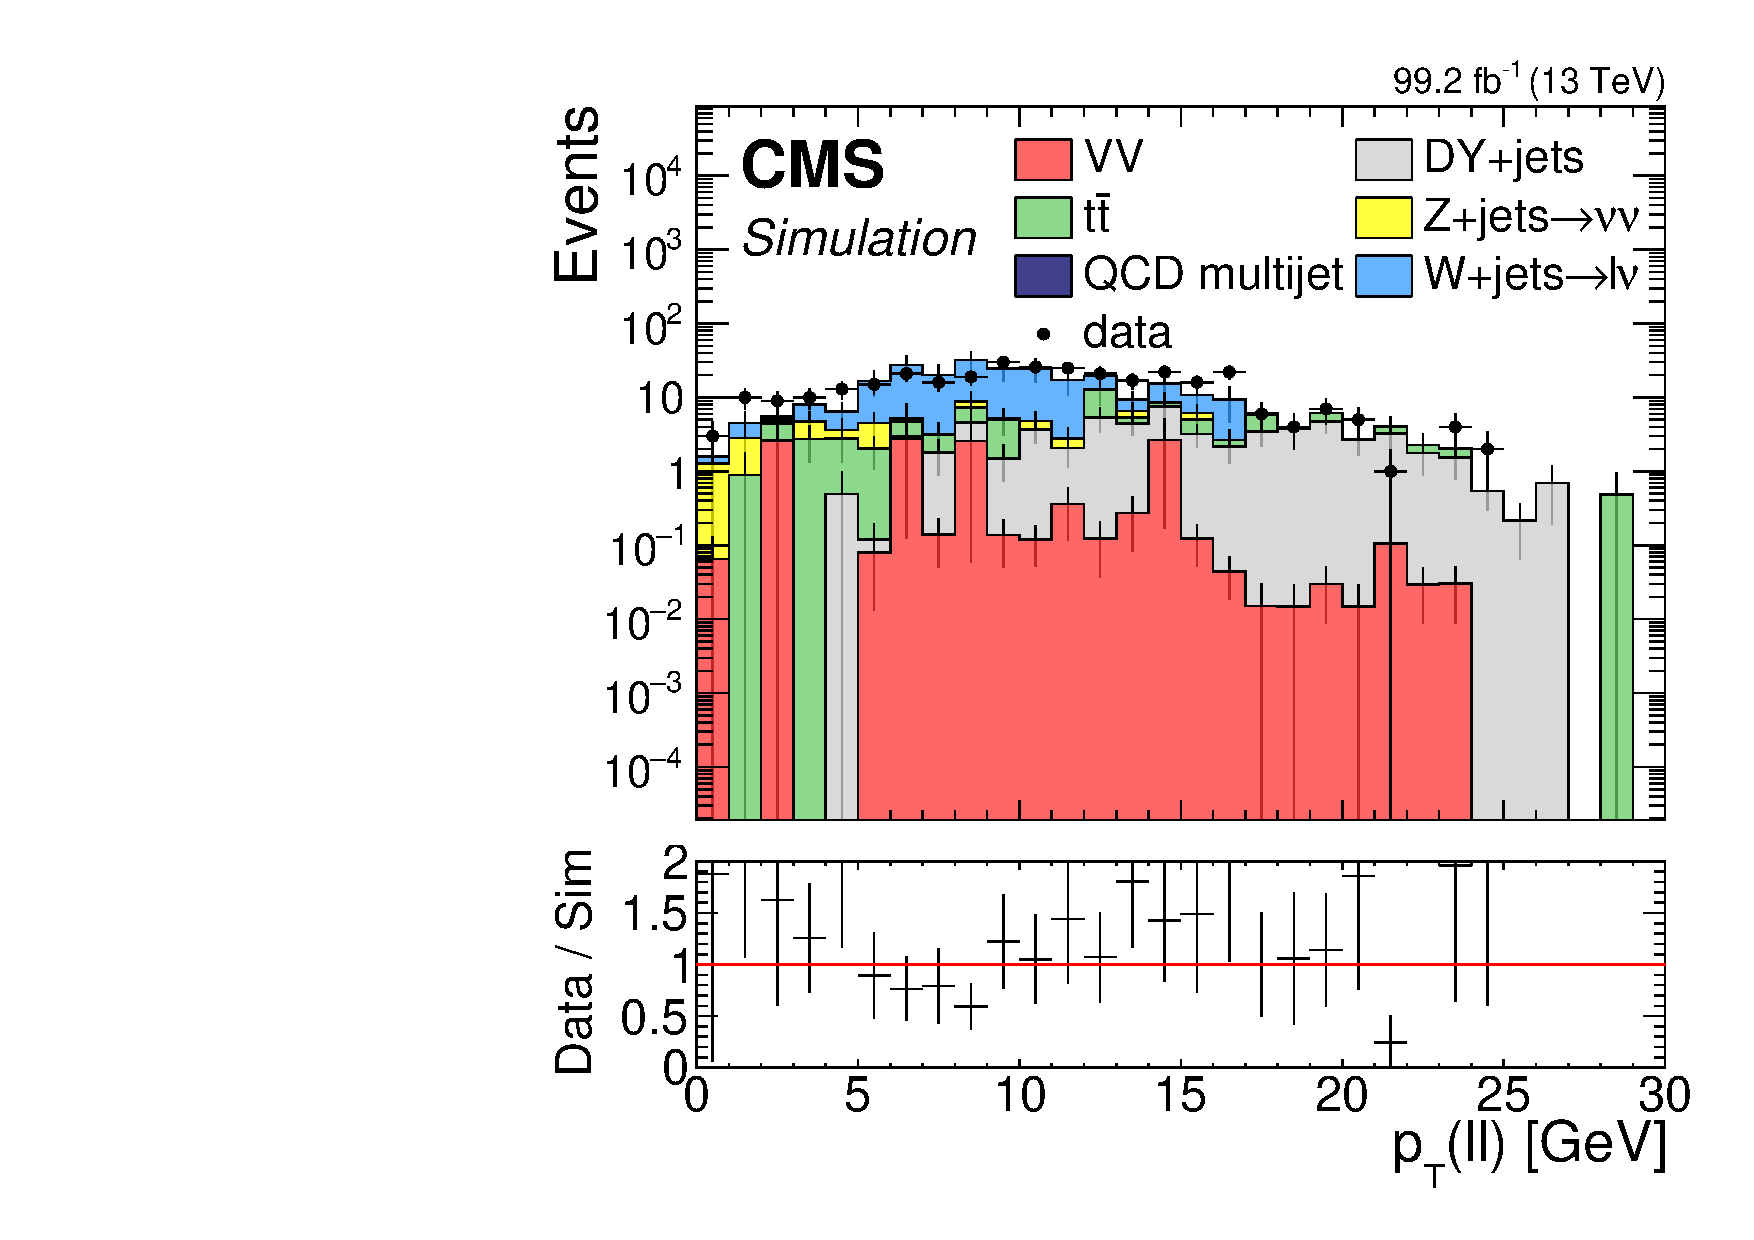
\includegraphics[width=0.48\linewidth]{plots/dilepton_muons_data_control_region_phase1/none_dileptonPtCorrJetNoMultIso10Dr0.6_log.pdf} \\

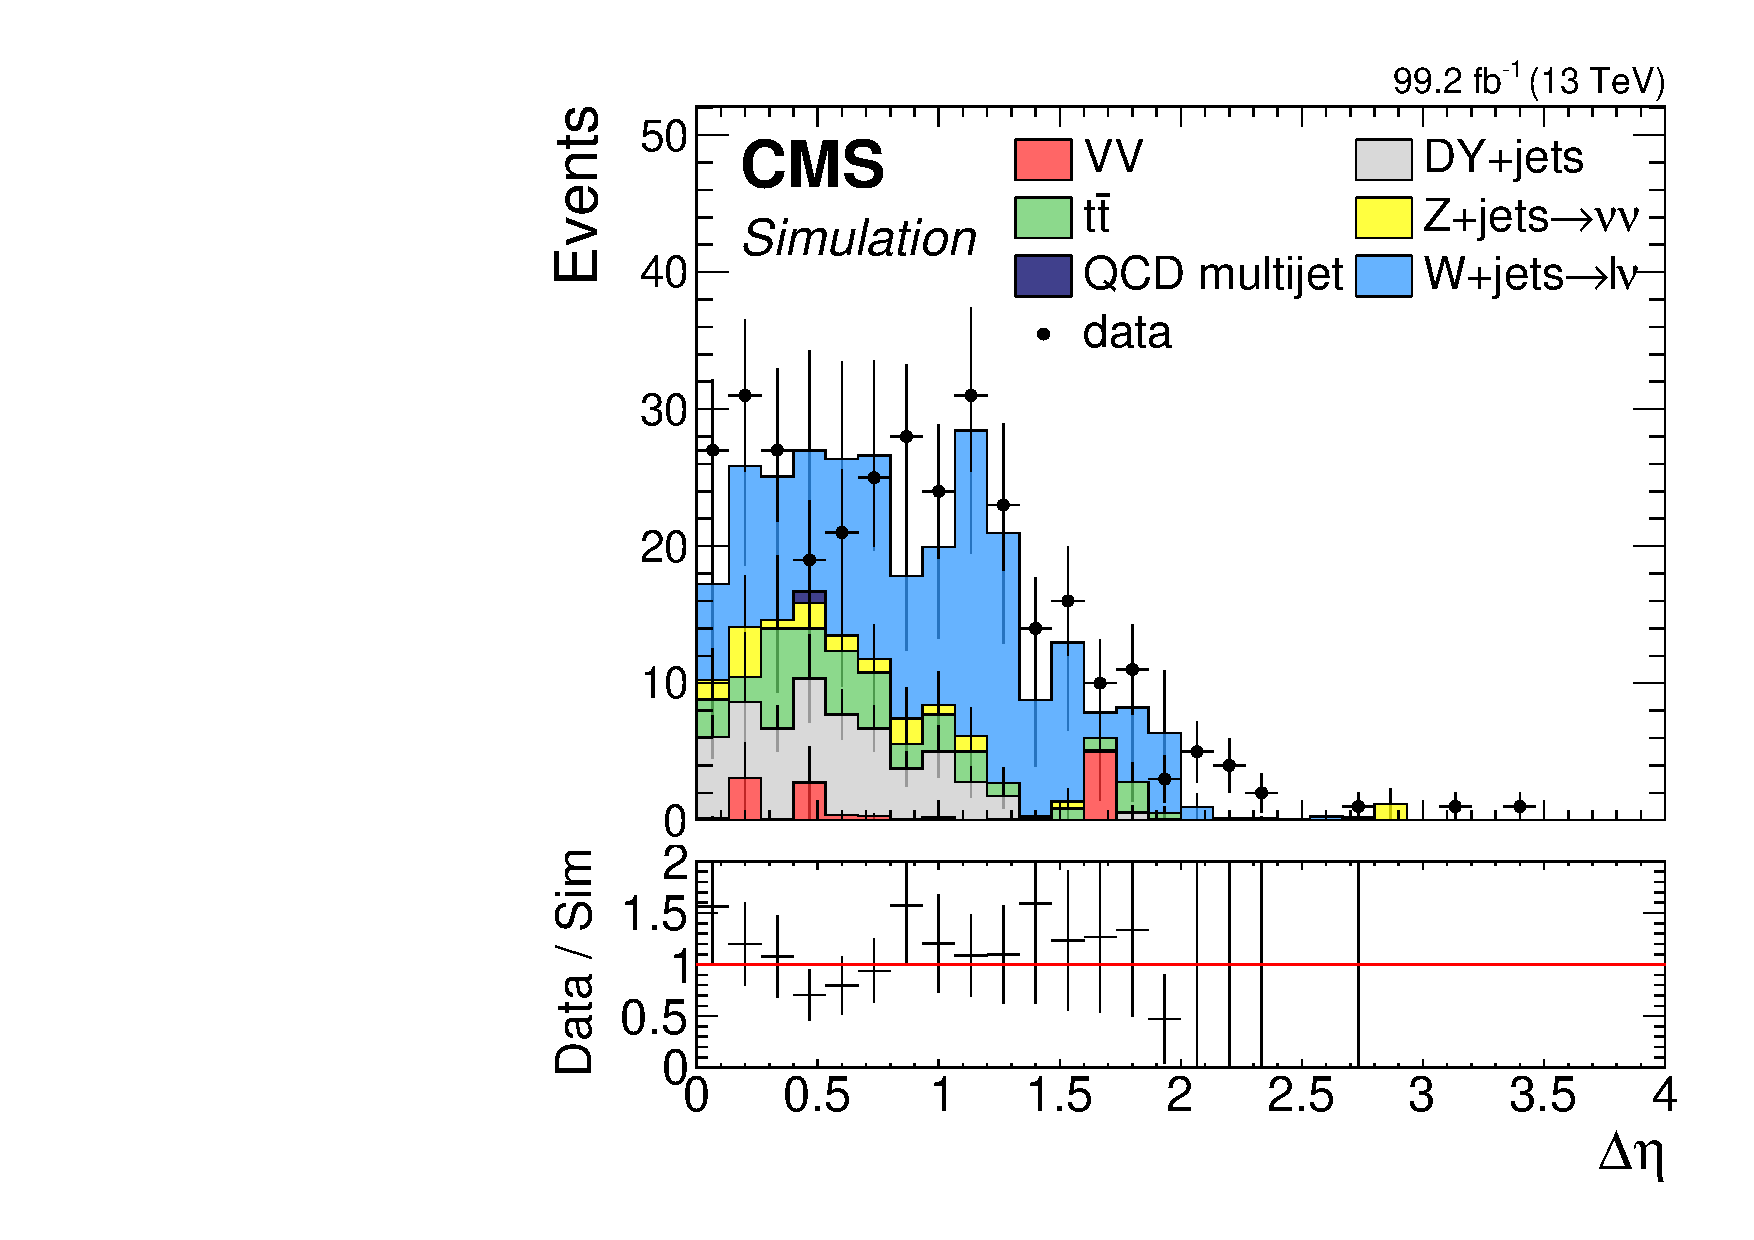
\includegraphics[width=0.48\linewidth]{plots/dilepton_muons_data_control_region_phase1/none_deltaEtaCorrJetNoMultIso10Dr0.6.pdf} \,
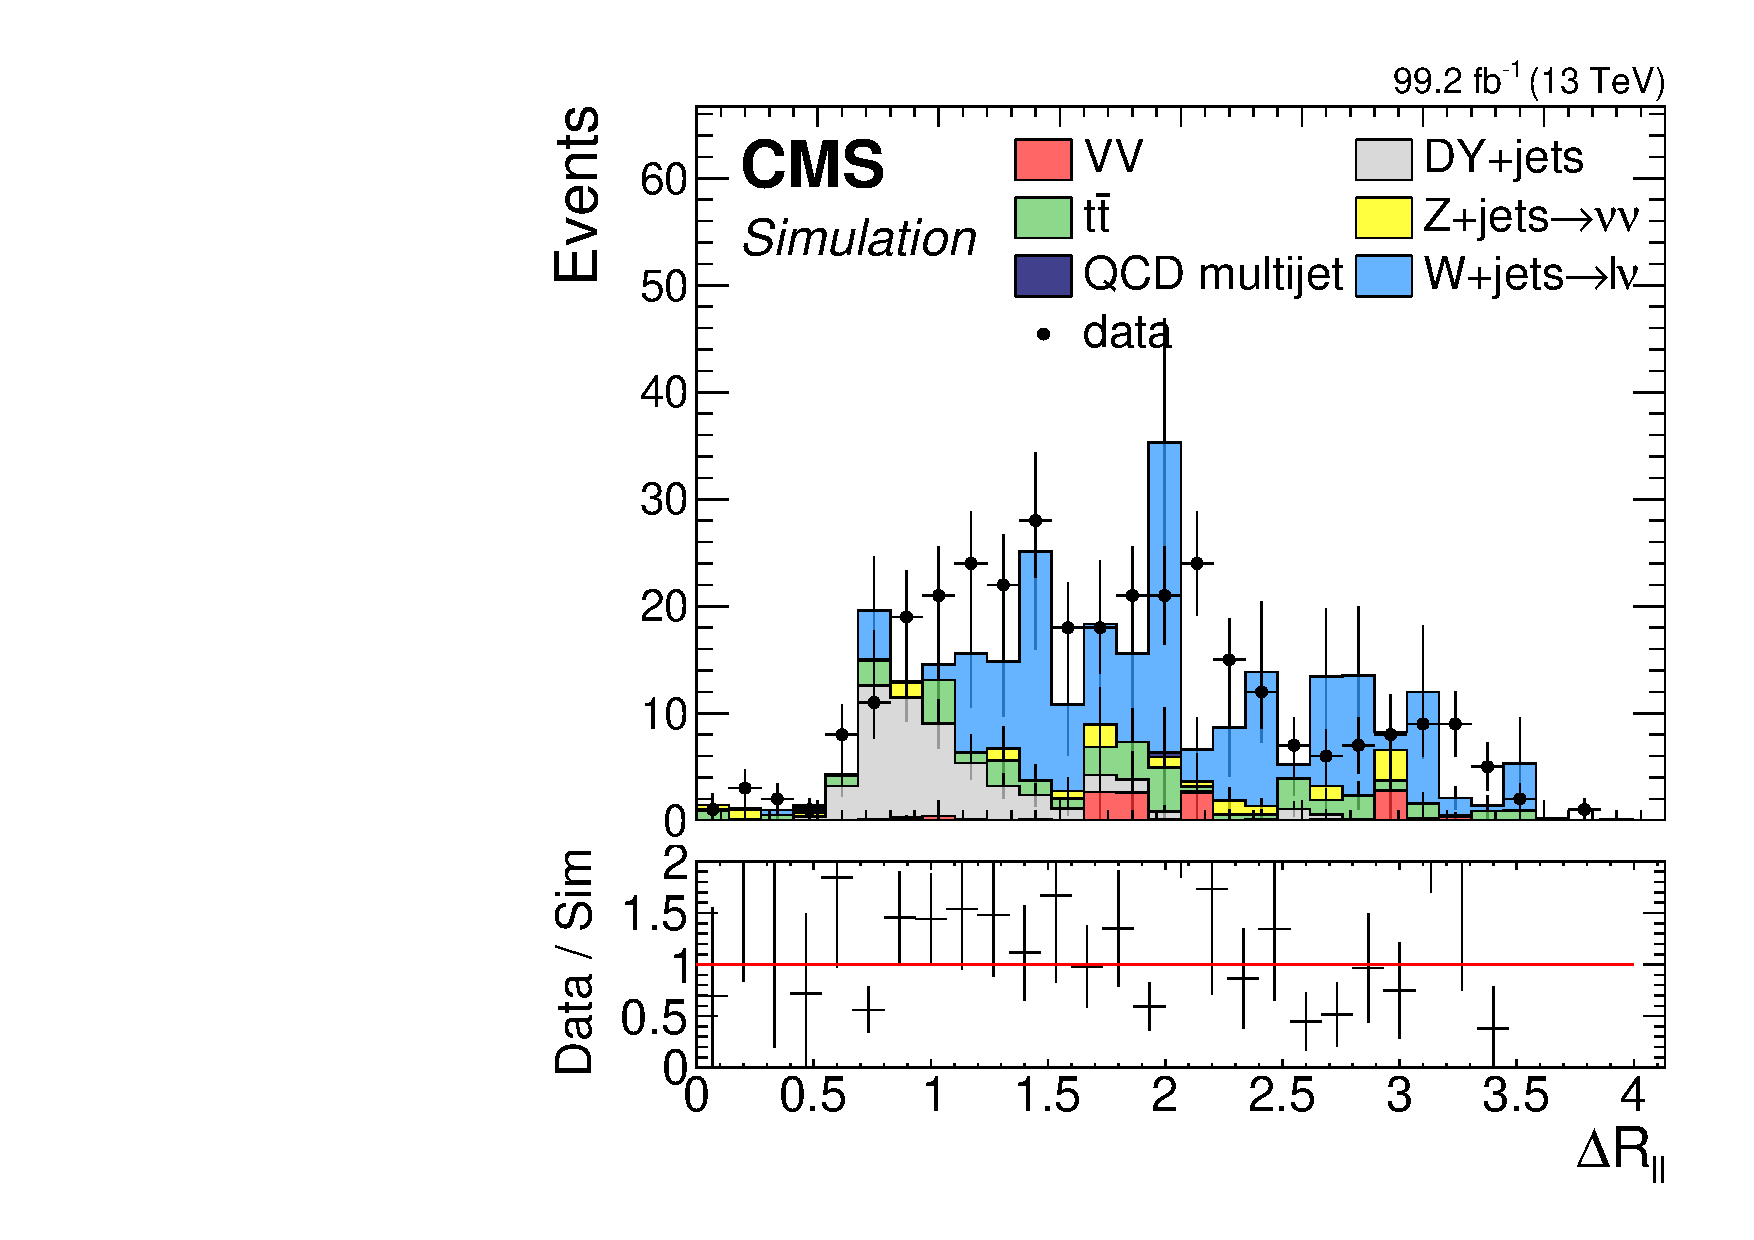
\includegraphics[width=0.48\linewidth]{plots/dilepton_muons_data_control_region_phase1/none_deltaRCorrJetNoMultIso10Dr0.6.pdf} \\

\end{figure} 